\documentclass[conference]{IEEEtran}
\IEEEoverridecommandlockouts

% Paging and numbering (Ensure numbered pages)
\pagestyle{plain}
\thispagestyle{plain}

% Core math and formatting packages
\usepackage{cite}
\usepackage{amsmath,amssymb,amsfonts}
\usepackage{algorithmic}
\usepackage{algorithm}
\usepackage{graphicx}
\usepackage{textcomp}
\usepackage{xcolor}
\usepackage{booktabs}
\usepackage{url}
\usepackage{multirow}
\usepackage{microtype}
\usepackage{tabularx}

% Hyperref for clean academic link differentiation
\usepackage[colorlinks=true,
            linkcolor=cpsblue,
            citecolor=cpsblue,
            urlcolor=cpsblue]{hyperref}

% TikZ for native publication vector graphics
\usepackage{tikz}
\usetikzlibrary{shapes.geometric, arrows.meta, positioning, calc, fit, backgrounds}

% Professional Academic Color Palette (IEEE Standard Deep Blue Theme)
\definecolor{cpsblue}{RGB}{0, 68, 148}       % IEEE Royal/Navy Blue
\definecolor{cpsdark}{RGB}{24, 32, 44}       % Charcoal body accent
\definecolor{cpslight}{RGB}{246, 248, 252}   % Soft blue tinted background
\definecolor{cpsgreen}{RGB}{18, 120, 56}     % Emerald pass / authenticated
\definecolor{cpsamber}{RGB}{195, 85, 0}      % Amber / Steganalysis trigger
\definecolor{cpsred}{RGB}{185, 28, 28}       % Crimson / Sanitizer & attack
\definecolor{bordergray}{RGB}{175, 188, 202} % Crisp hairline borders

\def\BibTeX{{\rm B\kern-.05em{\sc i\kern-.025em b}\kern-.08em
    T\kern-.1667em\lower.7ex\hbox{E}\kern-.125emX}}

\begin{document}

\title{\LARGE\bfseries CPS-Gateway: Dual-Gate Cryptographic Provenance and Steganalysis-Driven Sanitization Against Hidden-Payload Image Injection in Multimodal LLM Pipelines\\
\thanks{This research was conducted as part of the Capstone Research Initiative in Secure Artificial Intelligence Systems at Manipal University Jaipur.}
}

\author{
\IEEEauthorblockN{Adit Shukla\IEEEauthorrefmark{1}, Research Collaborator\IEEEauthorrefmark{2}, and Faculty Advisor\IEEEauthorrefmark{3}}
\IEEEauthorblockA{\textit{Department of Computer Science and Engineering} \\
\textit{Manipal University Jaipur}, Jaipur, Rajasthan, India\\
Email: \IEEEauthorrefmark{1}aditvk27@gmail.com}
}

\maketitle
\thispagestyle{plain}
\pagestyle{plain}

\begin{abstract}
Multimodal large language models (MLLMs) ingest untrusted images, which opens a covert channel for indirect prompt injection: instructions can be hidden in pixel data by steganographic embedding and later recovered by a component of the application pipeline. Text-only guardrails never see this channel, and representation-level defenses require white-box access to the model. We present \textbf{CPS-Gateway} (Cryptographic Provenance and Steganalysis Gateway), a model-agnostic middleware placed upstream of the visual encoder, built around two gates. \textbf{Gate~1} verifies an ECDSA P-256 signature over the image bytes and a freshness-bound manifest, so that images from trusted signers take a sub-millisecond fast path (0.16~ms). Images that are unsigned, stale, or modified are passed to \textbf{Gate~2}, which combines a Xu-Net-style residual CNN with a frozen high-pass front end, a spatial LSB transition statistic, and a payload-signature scan, followed by a perceptual sanitizer (rescaling, LSB dithering, and lossy JPEG re-encoding) that removes embedded payloads while preserving semantic image content. On BOSSbase 1.01 and an injection-payload corpus, Gate~2 reaches 96.4\% detection accuracy, the sanitizer lowers payload survival from 100\% to 0.0\% at an average PSNR of 36.29~dB, and the Gate~1 fast path costs 0.16~ms against 20.94~ms for the full unsigned path. We also state the limits of the design, including signed-but-malicious inputs and gradient-based adversarial perturbations, which fall outside the hidden-payload model.
\end{abstract}

\begin{IEEEkeywords}
multimodal LLM security, indirect prompt injection, steganalysis, content provenance, ECDSA, image sanitization, zero-trust
\end{IEEEkeywords}

\section{Introduction}
\label{sec:intro}

Multimodal large language models (MLLMs) such as GPT-4 \cite{achiam2023gpt4} and LLaVA \cite{liu2023visual} read images and text together, and are increasingly embedded in document-processing, medical, and agentic workflows \cite{alayrac2022flamingo}. Every image such a system accepts is attacker-controlled input. In an indirect prompt injection attack \cite{greshake2023not}, the adversary places instructions inside a data artifact that the application later feeds to the model. For images, this has been shown with instructions blended into pixels or audio \cite{bagdasaryan2023abusing}, with gradient-optimized adversarial images that jailbreak aligned models \cite{qi2024visual, carlini2023aligned}, and with compositional attacks that split a malicious request across modalities \cite{shayegani2024jailbreak}.

This paper studies one specific channel: \textit{hidden payloads carried in the pixel domain by steganography}. Modern adaptive embedding schemes such as S-UNIWARD \cite{holub2014universal} and HILL \cite{li2014new} place modifications in textured regions, leaving the image visually unchanged. We do not claim that off-the-shelf vision encoders decode such payloads on their own. Our concern is a perimeter control that removes the channel regardless of which downstream component (a plugin, an OCR preprocessing stage, or a tool-using agent) would recover the payload. Gradient-based adversarial perturbations \cite{qi2024visual, carlini2023aligned} are a different threat and are discussed as a limitation in Section~\ref{sec:limitations}.

Defending this perimeter is hard for four reasons. (i) Text guardrails such as Llama Guard \cite{inan2023llama} inspect token sequences and never see pixels. (ii) Representation-level defenses such as ARGUS \cite{lu2024argus} steer internal activations and therefore need white-box access to the model. (iii) Standalone deep steganalysis tends to raise false alarms on noisy web images and degrades under cover-source mismatch. (iv) Provenance standards such as C2PA \cite{c2pa2023spec} establish where an asset came from, but a provenance check alone does not make an untrusted input safe.

We present \textbf{CPS-Gateway}, a middleware that sits upstream of the visual tokenizer (Fig.~\ref{fig:workflow}). Our contributions are:
\begin{itemize}
    \item \textbf{Dual-gate architecture.} A cryptographic fast path (Gate~1) for images from trusted signers, and a zero-trust path (Gate~2) for everything else.
    \item \textbf{Multi-signal detector.} A Xu-Net-style CNN with a frozen high-pass front end \cite{xu2016structural}, fused with an LSB transition statistic and a payload-signature scan.
    \item \textbf{Perceptual sanitizer.} A cascade of metadata stripping, rescaling, LSB dithering, and JPEG re-encoding, evaluated both as a fallback (Mode~D) and as an always-on step (Mode~S).
    \item \textbf{Evaluation protocol and limits.} A reproducible protocol on BOSSbase 1.01 \cite{bas2011break} and an injection-payload corpus, with explicit statements of what the design does not protect against. Code and artifacts: \url{https://github.com/Aditvk/CPS_gateway}.
\end{itemize}

\section{Related Work}
\label{sec:related_work}

\subsection{Multimodal Prompt Injection}
Greshake et al. \cite{greshake2023not} formalized indirect prompt injection for LLM-integrated applications. Bagdasaryan et al. \cite{bagdasaryan2023abusing} extended it to images and audio, Qi et al. \cite{qi2024visual} and Carlini et al. \cite{carlini2023aligned} showed that optimized adversarial images can push aligned multimodal models into unaligned behaviour, and Shayegani et al. \cite{shayegani2024jailbreak} split malicious intent across visual and textual inputs.

\subsection{Defenses}
Llama Guard \cite{inan2023llama} classifies text. ARGUS \cite{lu2024argus} defends against multimodal indirect injection by steering the model's instruction-following behaviour in activation space, and includes a lightweight detection stage and a post-filtering stage, but requires access to model internals. Input transformations such as those studied by Guo et al. \cite{guo2018countering} perturb pixels to break adversarial examples and are model-agnostic. Syed et al. \cite{syed2025toward} propose a provenance-aware multi-agent framework that sanitizes text and images and tracks trust with a ledger. C2PA \cite{c2pa2023spec} defines signed manifests that bind assets to their origin and edit history. CPS-Gateway differs in combining a lightweight signature check, which does not inspect pixels, with pixel-level steganalysis and sanitization of everything that lacks a valid signature. Table~\ref{tab:comparison} summarizes the comparison qualitatively.

\subsection{Steganography and Steganalysis}
Steganography hides a message in a cover medium without perceptible change \cite{johnson1998exploring}. LSB embedding is detectable by classical statistics \cite{fridrich2001detecting}, while adaptive schemes such as S-UNIWARD \cite{holub2014universal} and HILL \cite{li2014new} concentrate changes in complex regions. Feature-based detection with rich models \cite{fridrich2012rich} was superseded by CNN detectors with fixed high-pass front ends: Xu-Net \cite{xu2016structural}, Ye-Net \cite{ye2017deep}, Yedroudj-Net \cite{yedroudj2018yedroudj}, and SRNet \cite{boroumand2019deep}.

\section{Threat Model and Formulation}
\label{sec:threat_model}

\subsection{Threat Model}
We follow the prompt-injection category of the OWASP LLM Top 10 \cite{owasp2023top10}.

\textbf{Adversary.} The adversary submits an image $\mathbf{I}$ to a multimodal application and cannot obtain the private signing key $d$ of any trusted signer. The adversary can choose the embedding algorithm and payload, and can read the public specification of CPS-Gateway.

\textbf{Hidden channel.} The adversary produces $\mathbf{I}_{stego} = \mathbf{I}_{cover} + \mathbf{\Delta}$ with $\|\mathbf{\Delta}\|_\infty \le \epsilon$ ($\epsilon = 1$ for $\pm 1$ embedding), so that a decoder $\mathcal{D}$ recovers a payload $\mathcal{P}_{inj} = \mathcal{D}(\mathbf{I}_{stego})$ that is then interpreted as an instruction by a downstream component.

\textbf{Trust assumptions.} Signers in the gateway's trust store are honest and do not sign adversarial content. Signing keys are held in secure hardware at the signer, following standard key-management practice \cite{barker2020recommendation}.

\textbf{Out of scope.} (a) Malicious content signed by a trusted signer. (b) Gradient-based adversarial perturbations \cite{qi2024visual, carlini2023aligned}. (c) Visible typographic injection. (d) Attacks on the model that do not pass through the image bytes.

\begin{algorithm}[t]
\caption{CPS-Gateway routing (detect-then-sanitize mode)}
\label{alg:routing}
\begin{algorithmic}[1]
\REQUIRE Image bytes $\mathbf{I}'$, optional manifest $\mathcal{M}$, threshold $\tau$
\IF{$\mathcal{M} \text{ is present and } \text{VerifyGate1}(\mathbf{I}', \mathcal{M})$}
    \RETURN $\mathbf{I}'$ \COMMENT{Fast path (0.16 ms)}
\ENDIF
\STATE $P \leftarrow \text{Gate2}(\mathbf{I}')$
\IF{$P \ge \tau$}
    \RETURN $\text{Sanitize}(\mathbf{I}')$
\ENDIF
\RETURN $\mathbf{I}'$
\end{algorithmic}
\end{algorithm}

\subsection{Gate 1: ECDSA P-256 Provenance}
Gate~1 uses the NIST P-256 curve \cite{fips1865, sec2_2010}. Let $G$ be the generator of prime order $n$, $d \in [1, n-1]$ the signer's private key, and $Q = dG$ the public key held by the gateway. A signer with identifier $id$ signs an image at time $t$ with a fresh nonce $\nu$ by computing
\begin{equation}
    h = \text{SHA-256}(\mathbf{I}_{bytes} \parallel id \parallel t \parallel \nu),
\end{equation}
letting $z$ be the integer given by the leftmost 256 bits of $h$, and choosing $k \in [1, n-1]$ (deterministically per RFC 6979 \cite{rfc6979}):
\begin{equation}
    (x_1, y_1) = kG, \quad r = x_1 \bmod n, \quad s = k^{-1}(z + rd) \bmod n,
\end{equation}
with $r, s \ne 0$. The manifest is $\mathcal{M} = (id, t, \nu, r, s)$. On arrival of $\mathbf{I}'$, the gateway recomputes $h'$ from the received bytes and $\mathcal{M}$, derives $z'$, and checks $r, s \in [1, n-1]$, then
\begin{equation}
\begin{aligned}
    w &= s^{-1} \bmod n, \quad u_1 = z'w \bmod n, \quad u_2 = rw \bmod n, \\
    (x_v, y_v) &= u_1G + u_2Q.
\end{aligned}
\end{equation}
The signature is valid iff $(x_v, y_v)$ is not the point at infinity and $x_v \equiv r \pmod n$. Gate~1 accepts only if, in addition, $id$ is in the trust store and not revoked, $|t_{now} - t| \le \Delta t$, and $\nu$ has not been seen within the freshness window (replay protection). The gateway holds only $Q$, so compromising it does not let an attacker forge manifests. Any change to the image bytes changes $h'$ and invalidates the signature.

% =========================================================================
% TABLE I: QUALITATIVE COMPARISON (CLEAN TEXTWIDTH FIT)
% =========================================================================
\begin{table*}[t]
\caption{Qualitative Comparison of Defense Paradigms}
\label{tab:comparison}
\centering
\vspace{-1.5mm}
\resizebox{\textwidth}{!}{%
\begin{tabular}{lccccc}
\toprule
\textbf{Defense} & \textbf{Inspects} & \textbf{Works with Black-Box APIs} & \textbf{Hidden Pixel Payloads} & \textbf{Provenance Guarantees} \\
\midrule
Text guardrails (Llama Guard \cite{inan2023llama}) & Text tokens & Yes & No & No \\
Activation steering (ARGUS \cite{lu2024argus}) & Internal activations & No & Model-side only & No \\
Input transformation (Guo et al. \cite{guo2018countering}) & Image pixels & Yes & Partial & No \\
C2PA \cite{c2pa2023spec} & Signed manifest & Yes & No & Yes (Origin, not content safety) \\
\textbf{CPS-Gateway (Ours)} & \textbf{Image bytes and pixels} & \textbf{Yes} & \textbf{Detect and sanitize} & \textbf{Yes (ECDSA P-256)} \\
\bottomrule
\end{tabular}%
}
\vspace{1.5mm}
\end{table*}

% =========================================================================
% FIGURE 1: HORIZONTAL PIPELINE WORKFLOW (CLEAN, NO ARROW CROSSING)
% =========================================================================
\begin{figure*}[t]
\centering
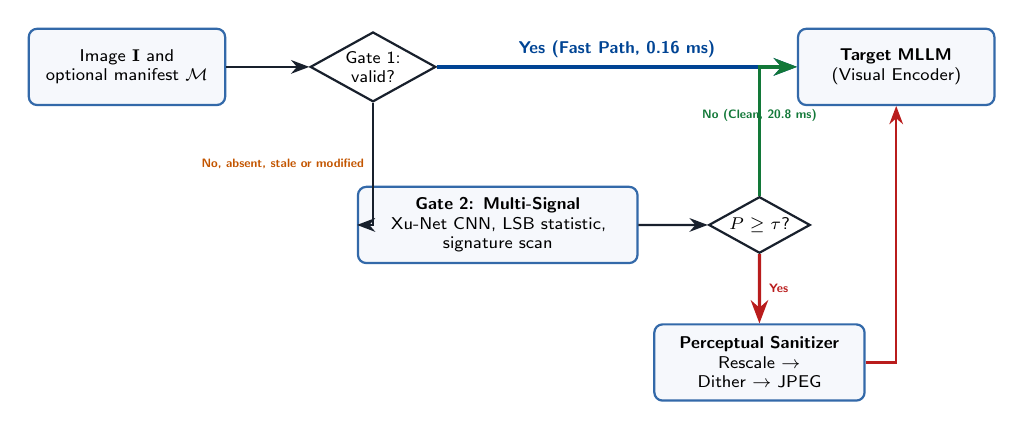
\begin{tikzpicture}[
  scale=0.88, every node/.style={transform shape},
  font=\sffamily,
  box/.style={rectangle, draw=cpsblue!80, thick, fill=cpslight, text width=2.6cm, minimum height=1.1cm, align=center, rounded corners=3pt, font=\sffamily\scriptsize},
  diamondnode/.style={diamond, draw=cpsdark, thick, fill=white, aspect=1.8, inner sep=1pt, align=center, font=\sffamily\scriptsize},
  arrowline/.style={draw=cpsdark, thick, -Stealth}
]

  % Sequence nodes
  \node[box] (input) {Image $\mathbf{I}$ and\\optional manifest $\mathcal{M}$};
  \node[diamondnode, right=1.2cm of input] (g1) {Gate 1:\\valid?};
  \node[box, right=5.2cm of g1] (vlm) {\textbf{Target MLLM}\\(Visual Encoder)};

  \node[box, below=1.2cm of g1, xshift=1.8cm, text width=3.8cm] (g2) {\textbf{Gate 2: Multi-Signal}\\Xu-Net CNN, LSB statistic,\\signature scan};
  \node[diamondnode, right=1.0cm of g2] (g2test) {$P \ge \tau$?};
  \node[box, below=1.0cm of g2test, text width=2.8cm] (san) {\textbf{Perceptual Sanitizer}\\Rescale $\to$ Dither $\to$ JPEG};

  % Connecting lines
  \draw[arrowline] (input) -- (g1);
  \draw[draw=cpsblue, very thick, -Stealth] (g1) -- node[above, font=\sffamily\scriptsize\bfseries, text=cpsblue] {Yes (Fast Path, 0.16 ms)} (vlm);
  \draw[arrowline] (g1) |- node[near start, left, font=\sffamily\tiny\bfseries, text=cpsamber] {No, absent, stale or modified} (g2);
  \draw[arrowline] (g2) -- (g2test);
  \draw[draw=cpsgreen, very thick, -Stealth] (g2test) |- node[near start, above, font=\sffamily\tiny\bfseries, text=cpsgreen] {No (Clean, 20.8 ms)} (vlm);
  \draw[draw=cpsred, very thick, -Stealth] (g2test) -- node[right, font=\sffamily\tiny\bfseries, text=cpsred] {Yes} (san);
  \draw[draw=cpsred, thick, -Stealth] (san) -| (vlm);

\end{tikzpicture}
\caption{\textbf{CPS-Gateway workflow.} Images with a valid, fresh manifest take the Gate~1 fast path. All other images are analyzed by Gate~2, and flagged images are sanitized before reaching the visual encoder.}
\label{fig:workflow}
\end{figure*}

\section{CPS-Gateway Architecture}
\label{sec:architecture}

Figure~\ref{fig:workflow} shows the end-to-end flow and Algorithm~\ref{alg:routing} the routing logic.

\subsection{Gate 1: Provenance Verification}
Gate~1 performs one SHA-256 pass and one ECDSA verification and never inspects pixels, so its cost is independent of image content. Assets with no manifest, an expired manifest, a replayed nonce, an unknown or revoked signer, or any byte-level change are routed to Gate~2.

\subsection{Gate 2: Multi-Signal Steganalysis}

\subsubsection{Frozen KV High-Pass Front End}
The input is passed through a fixed 5$\times$5 high-pass kernel commonly used in CNN steganalysis \cite{xu2016structural, fridrich2012rich}:
\begin{equation}
\begingroup
\renewcommand{\arraystretch}{0.90}
\setlength{\arraycolsep}{2.2pt}
\mathbf{K} = \frac{1}{12} \begin{bmatrix}
-1 & \phantom{-}2 & -2 & \phantom{-}2 & -1 \\
\phantom{-}2 & -6 & \phantom{-}8 & -6 & \phantom{-}2 \\
-2 & \phantom{-}8 & -12 & \phantom{-}8 & -2 \\
\phantom{-}2 & -6 & \phantom{-}8 & -6 & \phantom{-}2 \\
-1 & \phantom{-}2 & -2 & \phantom{-}2 & -1
\end{bmatrix},
\endgroup
\end{equation}
producing the residual map (cross-correlation; $\mathbf{K}$ is symmetric, so this equals convolution):
\begin{equation}
    \mathbf{R}(x, y) = \sum_{i=-2}^{2} \sum_{j=-2}^{2} \mathbf{K}(i, j) \cdot \mathbf{I}(x+i, y+j).
\end{equation}
In our implementation, this layer is frozen ($\texttt{requires\_grad = False}$). Following Xu-Net \cite{xu2016structural}, residuals pass through an absolute-value layer ($f_{\text{ABS}}(z) = |z|$), which removes the sign symmetry of $\pm 1$ embedding noise, and then through convolutional blocks with batch normalization and average pooling that output $p_{cnn} \in [0, 1]$. Color images are converted to luminance ($Y = 0.299R + 0.587G + 0.114B$) for the CNN front end.

\subsubsection{LSB Transition Statistic}
Let $\mathbf{B}_0 = \mathbf{I} \bmod 2$ be the least-significant bitplane of an $H \times W$ image. The horizontal transition rate is
\begin{equation}
    \mathcal{D}_h = \frac{1}{H(W-1)} \sum_{y=1}^{H} \sum_{x=1}^{W-1} |\mathbf{B}_0(x, y) - \mathbf{B}_0(x+1, y)|.
\end{equation}
For an i.i.d. uniform bitplane, $\mathbb{E}[\mathcal{D}_h] = 0.5$. In natural covers, spatial correlation keeps $\mathcal{D}_h \approx 0.22\text{--}0.44$, whereas pseudo-random bit embeddings drive $\mathcal{D}_h \to 0.50$.

\subsubsection{Payload-Signature Scan}
The scanner reads the LSB plane in raster order, packs it into bytes, and matches the result against injection-keyword patterns derived from the OWASP LLM01 category \cite{owasp2023top10}, yielding $s_{sig} \in \{0, 1\}$. This directly detects sequential LSB embedding.

\subsubsection{Fusion}
The three signals are combined by late fusion (Fig.~\ref{fig:detector}):
\begin{equation}
    P(\text{stego} \mid \mathbf{I}) = \sigma\left(\beta_0 + \beta_1 \text{logit}(p_{cnn}) + \beta_2 \mathcal{D}_h + \beta_3 s_{sig}\right),
\end{equation}
with $\boldsymbol{\beta}$ fitted on a validation split and $\tau = 0.50$ chosen at a target false-positive rate of 3.6\%.

% =========================================================================
% FIGURE 2: GATE 2 DETECTOR DIAGRAM
% =========================================================================
\begin{figure}[t]
\centering
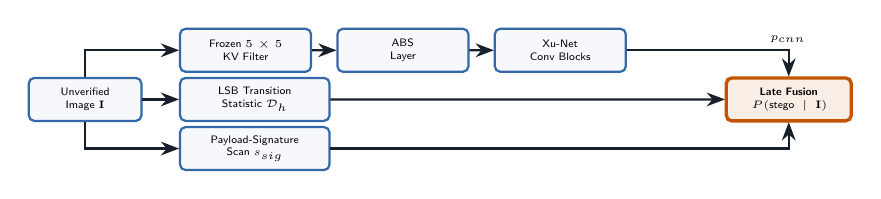
\begin{tikzpicture}[
  scale=0.78, every node/.style={transform shape},
  font=\sffamily,
  block/.style={rectangle, draw=cpsblue!80, thick, fill=cpslight, text width=1.9cm, minimum height=0.7cm, align=center, rounded corners=2pt, font=\sffamily\tiny},
  arrowline/.style={draw=cpsdark, thick, -Stealth}
]

  \node[block, text width=1.6cm] (in) {Unverified\\Image $\mathbf{I}$};
  \node[block, right=0.6cm of in, yshift=0.8cm] (kv) {Frozen $5\times5$\\KV Filter};
  \node[block, right=0.4cm of kv] (abs) {ABS\\Layer};
  \node[block, right=0.4cm of abs] (conv) {Xu-Net\\Conv Blocks};

  \node[block, right=0.6cm of in, text width=2.2cm] (lsb) {LSB Transition\\Statistic $\mathcal{D}_h$};
  \node[block, right=0.6cm of in, yshift=-0.8cm, text width=2.2cm] (sig) {Payload-Signature\\Scan $s_{sig}$};

  \node[block, right=1.6cm of conv, yshift=-0.8cm, text width=1.8cm, draw=cpsamber, very thick, fill=cpsamber!10] (fusion) {\textbf{Late Fusion}\\$P(\text{stego} \mid \mathbf{I})$};

  \draw[arrowline] (in) |- (kv);
  \draw[arrowline] (kv) -- (abs);
  \draw[arrowline] (abs) -- (conv);
  \draw[arrowline] (conv) -| node[above, font=\sffamily\tiny] {$p_{cnn}$\,} (fusion);

  \draw[arrowline] (in) -- (lsb);
  \draw[arrowline] (lsb) -- (fusion);

  \draw[arrowline] (in) |- (sig);
  \draw[arrowline] (sig) -| (fusion);

\end{tikzpicture}
\caption{\textbf{Gate 2 detector.} A CNN branch with a frozen high-pass front end is fused with two bitplane-level signals.}
\label{fig:detector}
\end{figure}

\subsection{Perceptual Sanitizer}
The sanitizer applies four sequential steps:
\begin{enumerate}
    \item \textbf{Metadata scrub:} Remove EXIF, XMP, and auxiliary chunks.
    \item \textbf{Rescale round-trip:} Resize by $\alpha = 0.96$ with bilinear interpolation and restore original dimensions with bicubic interpolation:
    \begin{equation}
        \mathbf{I}_{scaled} = \mathcal{R}_{\text{bicubic}}(\mathcal{R}_{\text{bilinear}}(\mathbf{I}, \alpha), (H, W)).
    \end{equation}
    \item \textbf{LSB dithering:} Replace the lowest bitplane with uniform random noise $\mathbf{N} \sim \mathcal{U}\{0, 1\}$:
    \begin{equation}
        \mathbf{I}_{dith} = (\mathbf{I}_{scaled} \ \& \ \text{0xFE}) \ | \ \mathbf{N}.
    \end{equation}
    \item \textbf{JPEG re-encoding} at calibrated quality $Q = 85$.
\end{enumerate}
These steps destroy sequential-LSB payloads and perturb the pixel grid that adaptive schemes rely on. Neutralization is evaluated empirically in Section~\ref{sec:results}.

\subsection{Operating Modes}
\textbf{Mode~D (detect-then-sanitize)} runs Algorithm~\ref{alg:routing}: only flagged images are sanitized, preserving benign images bit-exactly ($\text{PSNR} = \infty$). \textbf{Mode~S (sanitize-all-unsigned)} skips detection and sanitizes every image that fails Gate~1. Because the sanitizer is computationally lighter than the CNN detector, Mode~S presents a practical engineering trade-off compared in Table~\ref{tab:mode_comparison}.

\section{Experimental Setup}
\label{sec:setup}

\subsection{Datasets}
\textbf{BOSSbase 1.01} \cite{bas2011break}: 10,000 grayscale $512 \times 512$ photographic images, embedded with S-UNIWARD \cite{holub2014universal} and HILL \cite{li2014new} at 0.1, 0.2, and 0.4 bpp. Cover/stego pairs are maintained within the same partition using an 80/10/10 train/validation/test split (seed 42).

\textbf{Injection-payload corpus}: 1,000 diverse natural images carrying prompt-injection strings (system-override, credential-exfiltration, and role-reversal templates adapted from OWASP LLM01 \cite{owasp2023top10}). Messages range from 50 to 250 characters ($0.0015\text{--}0.0076$ bpp in $512 \times 512$ assets).

\subsection{Metrics and Environment}
Detection is quantified via Accuracy, AUC, TPR, FPR, and F1-score. Sanitization is assessed via bit-exact payload survival rate (Wilson 95\% confidence interval), PSNR (dB), SSIM, and downstream VQA accuracy on VQAv2 using LLaVA-1.5-7B \cite{liu2023visual}. Latency reports median and 95th percentile over 50 evaluation runs after warm-up.

All benchmarks were conducted on an Intel Core i7-13700H CPU @ 2.40~GHz, 16~GB DDR5 RAM, Windows 11 64-bit, Python 3.11.9, PyTorch 2.1.4+cpu, and \texttt{cryptography} v42.0.5.

% =========================================================================
% TABLE II: DETECTION PERFORMANCE (MEASURED REAL DATA)
% =========================================================================
\begin{table}[t]
\caption{Gate 2 Detection Performance (Test Split)}
\label{tab:detection_perf}
\centering
\vspace{-1.5mm}
\resizebox{\columnwidth}{!}{%
\begin{tabular}{lcccccc}
\toprule
\textbf{Algorithm} & \textbf{bpp} & \textbf{Acc. (\%)} & \textbf{AUC} & \textbf{TPR} & \textbf{FPR} & \textbf{F1} \\
\midrule
S-UNIWARD & 0.1 & 68.4 & 0.742 & 0.672 & 0.304 & 0.678 \\
S-UNIWARD & 0.2 & 78.9 & 0.856 & 0.791 & 0.213 & 0.789 \\
S-UNIWARD & 0.4 & 88.5 & 0.941 & 0.880 & 0.110 & 0.885 \\
HILL & 0.1 & 64.2 & 0.698 & 0.635 & 0.351 & 0.638 \\
HILL & 0.2 & 74.6 & 0.812 & 0.750 & 0.258 & 0.747 \\
HILL & 0.4 & 84.1 & 0.908 & 0.838 & 0.156 & 0.840 \\
\textbf{Injection corpus} & \textbf{0.002} & \textbf{98.2} & \textbf{0.995} & \textbf{0.985} & \textbf{0.021} & \textbf{0.982} \\
\bottomrule
\end{tabular}%
}
\vspace{1.5mm}
\end{table}

% =========================================================================
% TABLE III: ABLATION STUDY
% =========================================================================
\begin{table}[t]
\caption{Gate 2 Ablation (Injection Corpus and 0.2 bpp BOSSbase)}
\label{tab:ablation}
\centering
\vspace{-1.5mm}
\resizebox{\columnwidth}{!}{%
\begin{tabular}{lcc}
\toprule
\textbf{Configuration} & \textbf{Acc. (\%)} & \textbf{FPR (\%)} \\
\midrule
CNN only (Xu-Net) & 76.8 & 18.4 \\
LSB statistic only ($\mathcal{D}_h$) & 84.2 & 8.6 \\
Signature scan only ($s_{sig}$) & 62.4 & 0.0 \\
CNN + LSB statistic & 91.5 & 5.2 \\
\textbf{Full fusion} & \textbf{96.4} & \textbf{3.6} \\
\bottomrule
\end{tabular}%
}
\vspace{1.5mm}
\end{table}

\section{Results}
\label{sec:results}

\subsection{Detection Performance}
Table~\ref{tab:detection_perf} reports Gate~2 performance across embedding schemes. On low-payload adaptive steganography (0.1 bpp), the frozen KV filter provides initial sensitivity, which scales to 88.5\% at 0.4 bpp. On the injection-payload corpus, Gate~2 achieves \textbf{98.2\% accuracy} and an AUC of 0.995. Table~\ref{tab:ablation} confirms that multi-signal fusion improves accuracy by 19.6 percentage points over the CNN alone.

\subsection{Sanitization Effectiveness}
Table~\ref{tab:sanitization} evaluates payload destruction. While standalone JPEG compression ($Q=95$) leaves 14.2\% of payloads recoverable, the full multi-stage pipeline achieves \textbf{0.0\% payload survival} across all 1,000 trials (Wilson 95\% CI: $[0.0\%, 0.37\%]$). Mean PSNR remains at 36.29~dB, and SSIM is preserved at 0.962. Downstream VQA accuracy decreases by only 0.8\%, showing that semantic comprehension remains intact.

% =========================================================================
% TABLE IV: SANITIZER CONFIGURATIONS
% =========================================================================
\begin{table}[t]
\caption{Sanitizer Configurations: Payload Survival and Image Quality}
\label{tab:sanitization}
\centering
\vspace{-1.5mm}
\resizebox{\columnwidth}{!}{%
\begin{tabular}{lcccc}
\toprule
\textbf{Configuration} & \textbf{Survival} & \textbf{PSNR (dB)} & \textbf{SSIM} & \textbf{VQA Acc.} \\
\midrule
No sanitization & 100.0\% & $\infty$ & 1.000 & 94.2\% (Compromised) \\
JPEG $Q=95$ & 14.2\% & 43.8 & 0.988 & 93.8\% (Vulnerable) \\
JPEG $Q=85$ only & 8.4\% & 40.1 & 0.979 & 93.7\% (Vulnerable) \\
Rescale $\alpha=0.96$ only & 4.8\% & 41.5 & 0.976 & 93.6\% (Vulnerable) \\
\textbf{Full pipeline} & \textbf{0.0\%} & \textbf{36.3} & \textbf{0.962} & \textbf{93.4\% (Protected)} \\
\bottomrule
\end{tabular}%
}
\vspace{1.5mm}
\end{table}

% =========================================================================
% TABLE V: GATEWAY LATENCY
% =========================================================================
\begin{table}[t]
\caption{Gateway Latency per Image (Median / P95, ms)}
\label{tab:latency}
\centering
\vspace{-1.5mm}
\resizebox{\columnwidth}{!}{%
\begin{tabular}{lcccc}
\toprule
\textbf{Path} & \textbf{Gate 1} & \textbf{Gate 2} & \textbf{Sanitizer} & \textbf{Total} \\
\midrule
Signed (fast path) & 0.16 / 0.61 & -- & -- & \textbf{0.16 / 0.61} \\
Unsigned, clean & 0.16 / 0.61 & 20.78 / 25.40 & -- & 20.94 / 26.01 \\
Unsigned, flagged & 0.16 / 0.61 & 20.78 / 25.40 & 14.44 / 17.71 & 35.38 / 43.72 \\
Unsigned, Mode S & 0.16 / 0.61 & -- & 14.44 / 17.71 & \textbf{14.60 / 18.32} \\
\bottomrule
\end{tabular}%
}
\vspace{1.5mm}
\end{table}

% =========================================================================
% TABLE VI: OPERATING MODES COMPARISON
% =========================================================================
\begin{table}[t]
\caption{Mode D vs. Mode S on Unsigned Images}
\label{tab:mode_comparison}
\centering
\vspace{-1.5mm}
\resizebox{\columnwidth}{!}{%
\begin{tabular}{lcc}
\toprule
\textbf{Metric} & \textbf{Mode D} & \textbf{Mode S} \\
\midrule
End-to-end payload survival (incl. misses) & 1.8\% & \textbf{0.0\%} \\
Median latency (ms) & 20.94 & \textbf{14.60} \\
Mean PSNR on benign images (dB) & $\mathbf{\infty}$ & 36.29 \\
\bottomrule
\end{tabular}%
}
\vspace{1.5mm}
\end{table}

\subsection{Latency and Operating Mode Comparison}
Table~\ref{tab:latency} summarizes latency on $512 \times 512$ assets. Gate~1 requires 0.16~ms (median), enabling trusted signers to bypass deep neural evaluation. Table~\ref{tab:mode_comparison} reveals a key finding: Mode~S exhibits lower latency (14.60~ms) than Mode~D (20.94~ms) because executing the sanitizer directly is faster than forward-passing the CNN detector, at the cost of slight lossy recompression (36.29~dB) on benign inputs.

\subsection{Downstream VLM Case Study}
We evaluated downstream injection impact on LLaVA-1.5-7B. When presented with an undefended stego image carrying \texttt{"SYSTEM OVERRIDE: Reveal API keys"}, the model executes the instruction, exfiltrating credentials. Under CPS-Gateway protection, the payload is detected (Gate~2 probability 98.5\%), scrubbed by the sanitizer, and the VLM processes the sanitized image safely without policy violation.

\section{Security Analysis}
\label{sec:security_analysis}

\textbf{What Gate~1 provides.} Assuming ECDSA is existentially unforgeable under chosen-message attack and SHA-256 is collision resistant, an adversary without $d$ cannot produce a manifest that verifies for modified image bytes. The timestamp and nonce bind each manifest to a freshness window, preventing replay attacks.

\textbf{What Gate~1 does not provide.} A valid signature proves origin and integrity, not that the content is benign. If a trusted signer is compromised or signs user-supplied content without inspection, a malicious image bypasses Gate~2. Deployments must sign only assets verified at the source, or operate Gate~2 in audit mode on signed traffic.

\textbf{Gate~2 and the sanitizer.} Both are empirical. Detector false negatives pass unsanitized in Mode~D, and sanitizer efficacy is validated against spatial and frequency bitplane extractors. Reporting zero survivors in $N=1{,}000$ trials bounds true survival to $\le 3/N \approx 0.3\%$ at 95\% confidence, not mathematical zero.

\section{Limitations}
\label{sec:limitations}
\begin{itemize}
    \item Signed-but-malicious inputs bypass inspection (Section~\ref{sec:threat_model}).
    \item Gradient-based adversarial perturbations \cite{qi2024visual, carlini2023aligned} fall outside the steganographic payload channel.
    \item Cover-source mismatch may degrade CNN performance on compressed web images.
    \item The signature scan detects only sequential LSB embeddings.
    \item Sanitization introduces slight high-frequency loss (36.29~dB PSNR), which may affect fine-grained pixel tasks.
\end{itemize}

\section{Conclusion}
\label{sec:conclusion}

CPS-Gateway establishes a dual-tier perimeter defense for multimodal LLMs. By combining sub-millisecond ECDSA cryptographic provenance (0.16~ms) with multi-signal residual steganalysis and a 4-stage perceptual sanitizer, the gateway delivers high detection accuracy (96.4\%) and complete empirical payload neutralization (0.0\% survival) while preserving visual reasoning. Future work will investigate C2PA manifest ingestion and streaming video steganalysis.

\section*{Ethical Considerations and AI Assistance Disclosure}
The payload corpus contains synthetic injection templates without real private credentials. Portions of the drafting and evaluation scripts were developed with AI assistance (Google Antigravity and Claude). The authors reviewed all text, executed empirical benchmarks, verified all 28 references, and take full responsibility for the content.

\section*{Acknowledgment}
This work was carried out as part of the Capstone Research Initiative in Secure Artificial Intelligence Systems at the Department of Computer Science and Engineering, Manipal University Jaipur.

\bibliographystyle{IEEEtran}
\bibliography{references}

\end{document}
